%%%%%%%%%%%%%%%%%%%%%%%%%%%%%%%%%%%%%%%%%%%%%%%%%%%%%%%%
%%%%                                              %%%%%%
%%%%  Author: Peter Wilson                        %%%%%%
%%%%                                              %%%%%%
%%%%  Background of shells                        %%%%%%
%%%%                                              %%%%%%
%%%%%%%%%%%%%%%%%%%%%%%%%%%%%%%%%%%%%%%%%%%%%%%%%%%%%%%%

\chapter[Analytical membrane analysis of dome]{Analytical membrane\\ analysis of dome}
\label{app:Analytical membrane analysis of dome}
\renewcommand{\Thema}{Analytical membrane analysis of dome}

Forming the reference solution to the isotropic quantity recovery test presented in section \ref{subsection:dome_test}, the analytical membrane solution of a simply supported dome with an oculus under self weight is presented.

\begin{figure}[H]
	%\centering
	\subfloat[Rotationally symmetric shell geometry]
	{\label{ref_label1}
		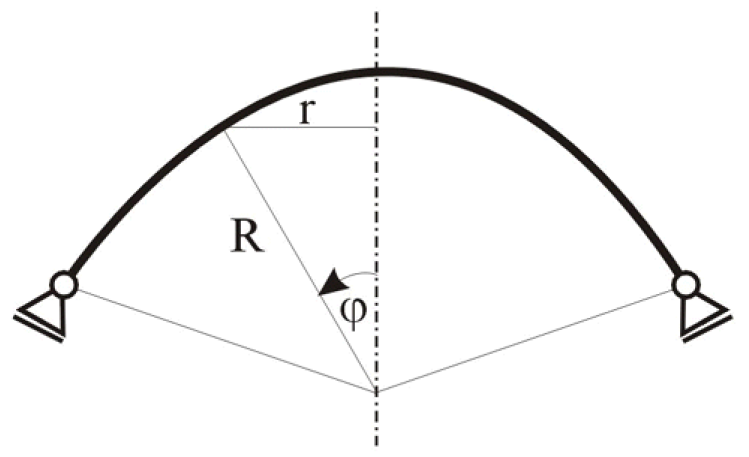
\includegraphics[width=7.3cm]
		{images/dome_geom.png}}
	\subfloat[Relation of self weight to normal and tangential pressures]
	{\label{ref_label2}
		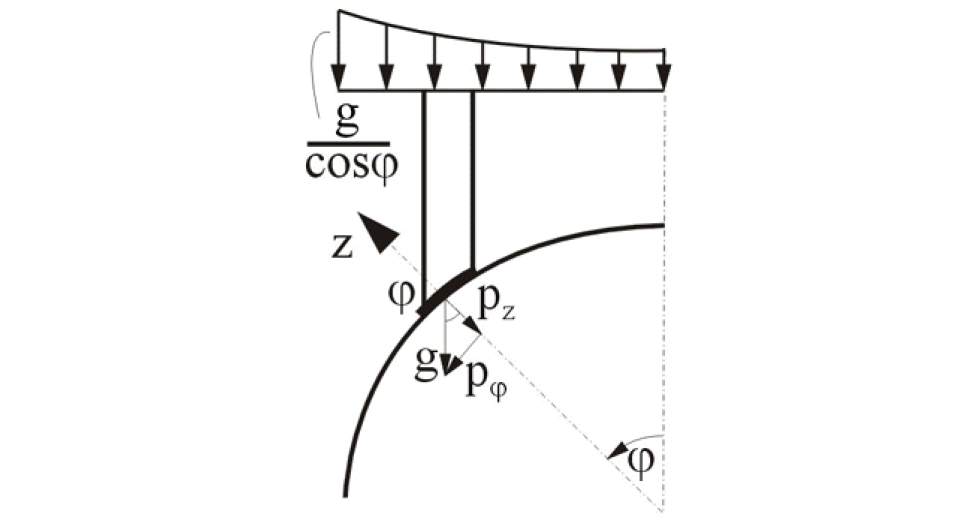
\includegraphics[width=7.3cm]
		{images/dome_self_weight.png}}
	\caption{\label{App3_dome}Dome geometry and loading}
\end{figure}

The self weight of a dome with uniform thickness $t$ and density $\rho$ is transferred into normal and tangential pressures as per the following formulae:

\begin{equation} 
p_\phi = \gamma t sin\phi\ ,
\hspace{10mm}
p_z = -\gamma t cos\phi
\hspace{10mm}
with
\hspace{10mm}
\gamma = \rho g
\label{eqapp3_1}\ .
\end{equation}

Fulfilling the special case of rotational symmetry, due to uniform thickness and density, the total support reaction $P_v$ of the dome with an oculus corresponding to $\phi_0 = 20^{\circ} = \frac{\pi}{9} rad$ can be determined as:

\begin{equation} 
P_v = 2\pi R^2 \int_{\phi_0 = \frac{\pi}{9}}^{\phi}
sin^3 \phi \ \gamma t + sin \phi \ cos^2 \phi \ \gamma t
\ d\phi + C
\label{eqapp3_2}\ .
\end{equation}
With no edge load along the oculus, C = 0. Simplifying and integrating yields:
\begin{equation} 
P_v = 2\pi R^2 \gamma t (cos\phi - cos \frac{\pi}{9})
\label{eqapp3_3}\ .
\end{equation}

With the total support reaction known, the meridional $n_\phi$ and circumferential $n_\theta$ force resultants can be determined at any meridional position $\phi$ with the following simplified expressions:

\begin{equation} 
n_\phi = \frac{R\gamma t (cos \phi \ - cos\frac{\pi}{9})}{sin^2\phi} 
\label{eqapp3_4}
\end{equation}
and
\begin{equation} 
n_\theta = -R \gamma t cos \phi \ - n_\phi
\label{eqapp3_5}\ .
\end{equation}